\documentclass[14pt]{extarticle}

\usepackage{geometry}
\usepackage{amsmath,amsthm,amssymb}
\usepackage[utf8]{inputenc}
\usepackage[T1,T2A]{fontenc}
\usepackage{bold-extra}
\usepackage[english,russian]{babel}
\usepackage{indentfirst}
\usepackage{graphicx}
\graphicspath{ {images/} }
\usepackage{float}
\usepackage{listings}
\usepackage{lmodern}
\usepackage{appendix}
\usepackage{braket}
\usepackage{cite}
\usepackage[nottoc,numbib]{tocbibind}

\geometry{
a4paper,
left = 20mm,
right = 15mm,
bottom = 20mm,
top = 20mm,
}
\renewcommand{\rmdefault}{ftm} % TimesNewRoman
\renewcommand{\baselinestretch}{1.5} 

\begin{document}

\begin{titlepage}
	\begin{center}
		\small{ФЕДЕРАЛЬНОЕ ГОСУДАРСТВЕННОЕ БЮДЖЕТНОЕ ОБРАЗОВАТЕЛЬНОЕ}\\ 
			УЧРЕЖДЕНИЕ ВЫСШЕГО ОБРАЗОВАНИЯ\\
			«МОСКОВСКИЙ ГОСУДАРСТВЕННЫЙ УНИВЕРСИТЕТ\\
			имени М.В.ЛОМОНОСОВА»\\
		\hfill \break
		ФАКУЛЬТЕТ ВЫЧИСЛИТЕЛЬНОЙ МАТЕМАТИКИ И КИБЕРНЕТИКИ\\
		КАФЕДРА СУПЕРКОМПЬЮТЕРОВ И КВАНТОВОЙ ИНФОРМАТИКИ\\
		\vfill
		ОТЧЁТ \\
		\textbf{<<АНАЛИЗ АЛГОРИТМА СОРТИРОВКИ СЛИЯНИЕМ>>}\\
	\end{center}	
	\vfill
	\begin{flushright}
		Выполнил студент \\
		группы м118:\\
		Пухов Д. Н.\\
		{\hspace{3cm}}
	\end{flushright}
	
	
	\begin{center}
		Москва \\
		2017 
	\end{center}
	
	\thispagestyle{empty}

\end{titlepage}



\section*{Формулировка задачи} 
Реализовать последовательный алгоритм сортировки слиянием, исследовать его теоретическую производительность и практическую производительность, а именно получить число сравнений данных, число копирований данных, амортизационный коэффициент алгоритма и время работы алгоритма в зависимости от размера входных данных. Также рассмотреть оптимизацию алгоритма для малых массивов.

\section*{Описание алгоритма}
Классический алгоритм сортировки слиянием выглядит следующим образом:

\begin{lstlisting}
mergesort(array):
	if array length == 1, return
	mergesort(left half of array)
	mergesort(right half of array)
	merge(left half of array, right half of array)
\end{lstlisting}
Наиболее интересная часть алгоритма --- процедура слияния двух массивов. Простейшая её реализация использует дополнительную память, необходимую для хранения результата.

\section*{Анализ производительности}

\subsection*{Слияние}

На вход процедура получает указатель на массив, длину его левой и длину правой рассортированных по возрастанию частей (это не обязательно половины). Выделяется память для хранения массива, полученного слиянием данных массивов (по их общей длине), т.н. буфер. Затем начинается непосредственно слияние: выбирается минимальный элемент из левой и правой частей и копируется в буфер, соответствующая часть массива укорачивается на один элемент. Эта операция делается в 2 шага: сравнение первых элементов (достаточно выбирать только из первых элементов, поскольку массивы рассортированы) и перемещение этого элемента. Процедура повторяется, пока один из массивов не окажется пустым. Оставшийся массив просто копируется в буфер. Затем буфер копируется в исходный массив.

\begin{figure}[H]
	\centering
	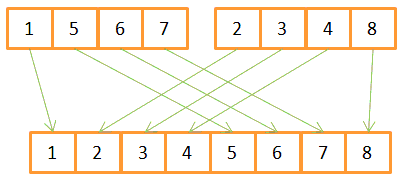
\includegraphics[scale=1]{merge}
\end{figure}

Пусть левая часть имеет размер $n$, правая - $m$.
Очевидно, что требуется $ min(n, m) $ до $ max(n, m) $ сравнений и $ 2(n+m) $ копирований. То есть сложность алгоритма линейная, $ O(n+m) $.

Можно заметить, что не требуется выдлеять под буфер $n+m$ памяти, достаточно только $n$ --- сначала копируем левую часть массива, затем производим слияние сразу в исходный массив.
Тогда оценка копирований изменится: от $2n$ до $2n+m$. В среднем число копирований будет ближе к верхней границе, поскольку нижняя граница достижима лишь в случае, когда минимальный элемент правой части массива больше максимального элемента левой части массива, что на случайных данных при большой длине массива и малом диапазоне чисел крайне маловероятно.

В случае деления пополам ($m=n=N/2$) имеем: от $N$ до $ 1.5 N $ копирований и от $0.5 N$ до $N$ сравнений.

\subsection*{Сортировка}
Алгоритм сортировки слиянием использует стратегию "разделяй и властвуй". Запишем рекурсивную формулу для времени его выполнения в случае деления массива пополам: $ T(N) \le 2T(N/2) + \alpha N \le 4T(N/4) + 2 \alpha N \le ... \le N \cdot T(1) + \alpha N log N = \Theta (N log N)$. Это оценка сверху. Справедлива ровно такая же оценка снизу с другим коэффициентом $ \beta $ в силу линейной сложности слияния. Таким образом, получаем, что $ T(N) = \Theta(N log N) $. Это значит, что алгоритм не имеет сложных входных данных. Однако на рассортированном массиве алгоритм работает почти так же долго, как и на случайном.

\begin{figure}[H]
	\centering
	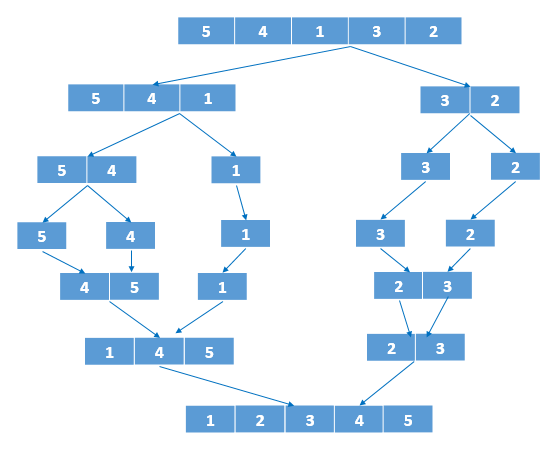
\includegraphics[scale=1]{mergesort}
\end{figure}

Общее число сравнений: в лучшем случае $ 0.5 N log N $, в худшем --- $ N log N $.

Общее число копирований: в лучшем случае $ N log N $, в худшем --- $ 1.5 N log N $.

\subsection*{Оптимизация для малых массивов}
Можно заметить, что при работе с малыми массивами сортировка слиянием делает много лишней работы, а именно: функция вызывается и ничего не делает, когда размер массива меньше двух. Вызов функции --- сравнительно недешёвая операция, и в данном случае логично для малых массивов использовать более простую сортировку, например, сортировку вставками. В худшем случае она несильно проигрывает сортировке слиянием (на малых массивах, разумеется), а в лучшем сильно её опережает (на отсортированном массиве сортировка вставками делает всего лишь N копирований и N сравнений). Длина массива, при которой массив можно считать маленьким, зависит от архитектуры конкретного компьютера, обычно колеблясь между 8 и 30 элементами.

\section*{Результаты}
Были проведены измерения для неоптимизированной сортировки слиянием (на картинках именуется как plain) и для оптимизированной (merge) на процессоре Intel Core i5 3230M. Размер входных данных изменялся от 100 до нескольких миллиардов элементов, увеличиваясь вдвое. Данные для сортировки были получены с помощью генератора псевдослучайных чисел из стандартной библиотеки языка Си. Сортировался тип char (ввиду его малого размера). Данные получены без усреднения.

На первом графике изображено время работы алгоритмов, делённое на длину массива. Ожидаемая зависимость --- log N. В полулогарифмическом масштабе это прямая, что и наблюдаем. Однако при малых размерах неоптимизированная сортировка слиянием ведёт себя довольно хаотично и имеет бОльшее время выполнения.

На втором графике показана зависимость коэффициента амортизации алгоритма от размера входных данных. Ожидается, что с увеличением размера входных данных этот коэффициент выходит на асимптоту (здесь около 6).

На третьем и четвёртом графиках показано число сравнений и число копирований элементов, делённые на размер массива. Как и в случае со временем, ожидаем увидеть прямую (логарифм в полулогарифмическом масштабе). Видно, что реализуются худший случай и в числе обменов, и в числе копирований. Объяснение этого эффекта найти, однако, не удаётся.

\begin{figure}[H]
	\centering
	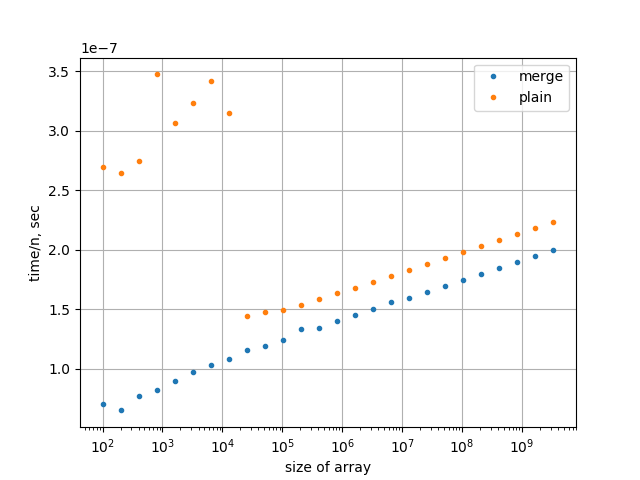
\includegraphics[scale=1]{Figure_3}
\end{figure}

\begin{figure}[H]
	\centering
	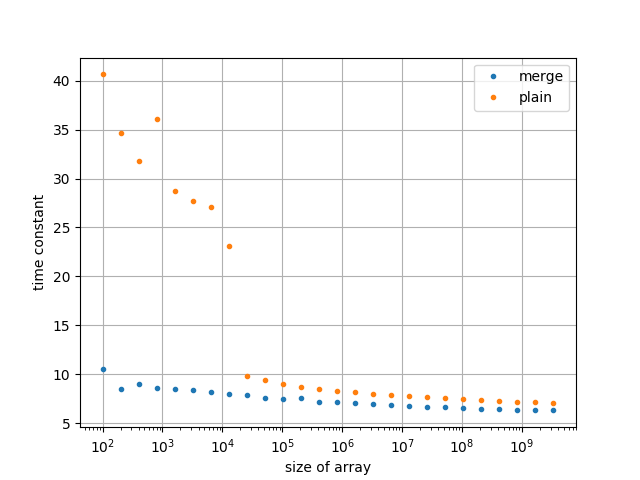
\includegraphics[scale=1]{Figure_4}
\end{figure}

\begin{figure}[H]
	\centering
	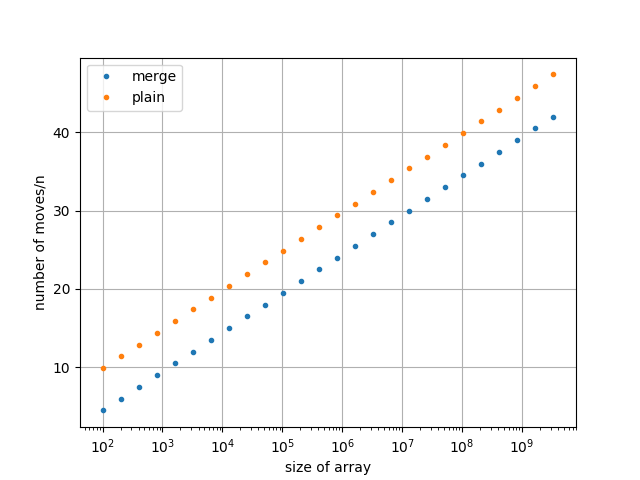
\includegraphics[scale=1]{Figure_1}
\end{figure}

\begin{figure}[H]
	\centering
	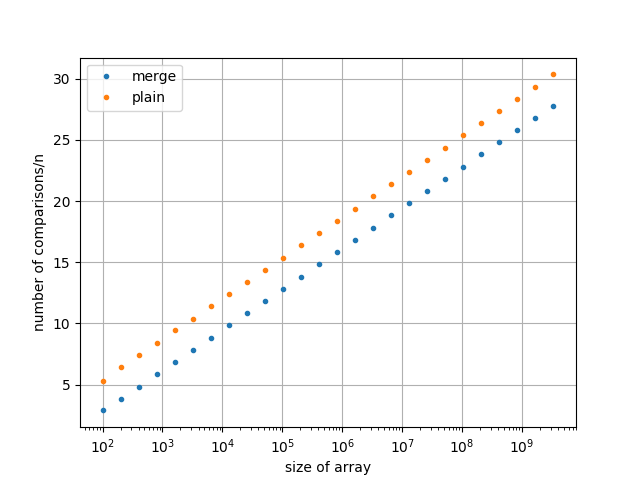
\includegraphics[scale=1]{Figure_2}
\end{figure}


\end{document}\grid
